\newpage
\section{GPU reduction: naive}
\begin{figure}[h]
    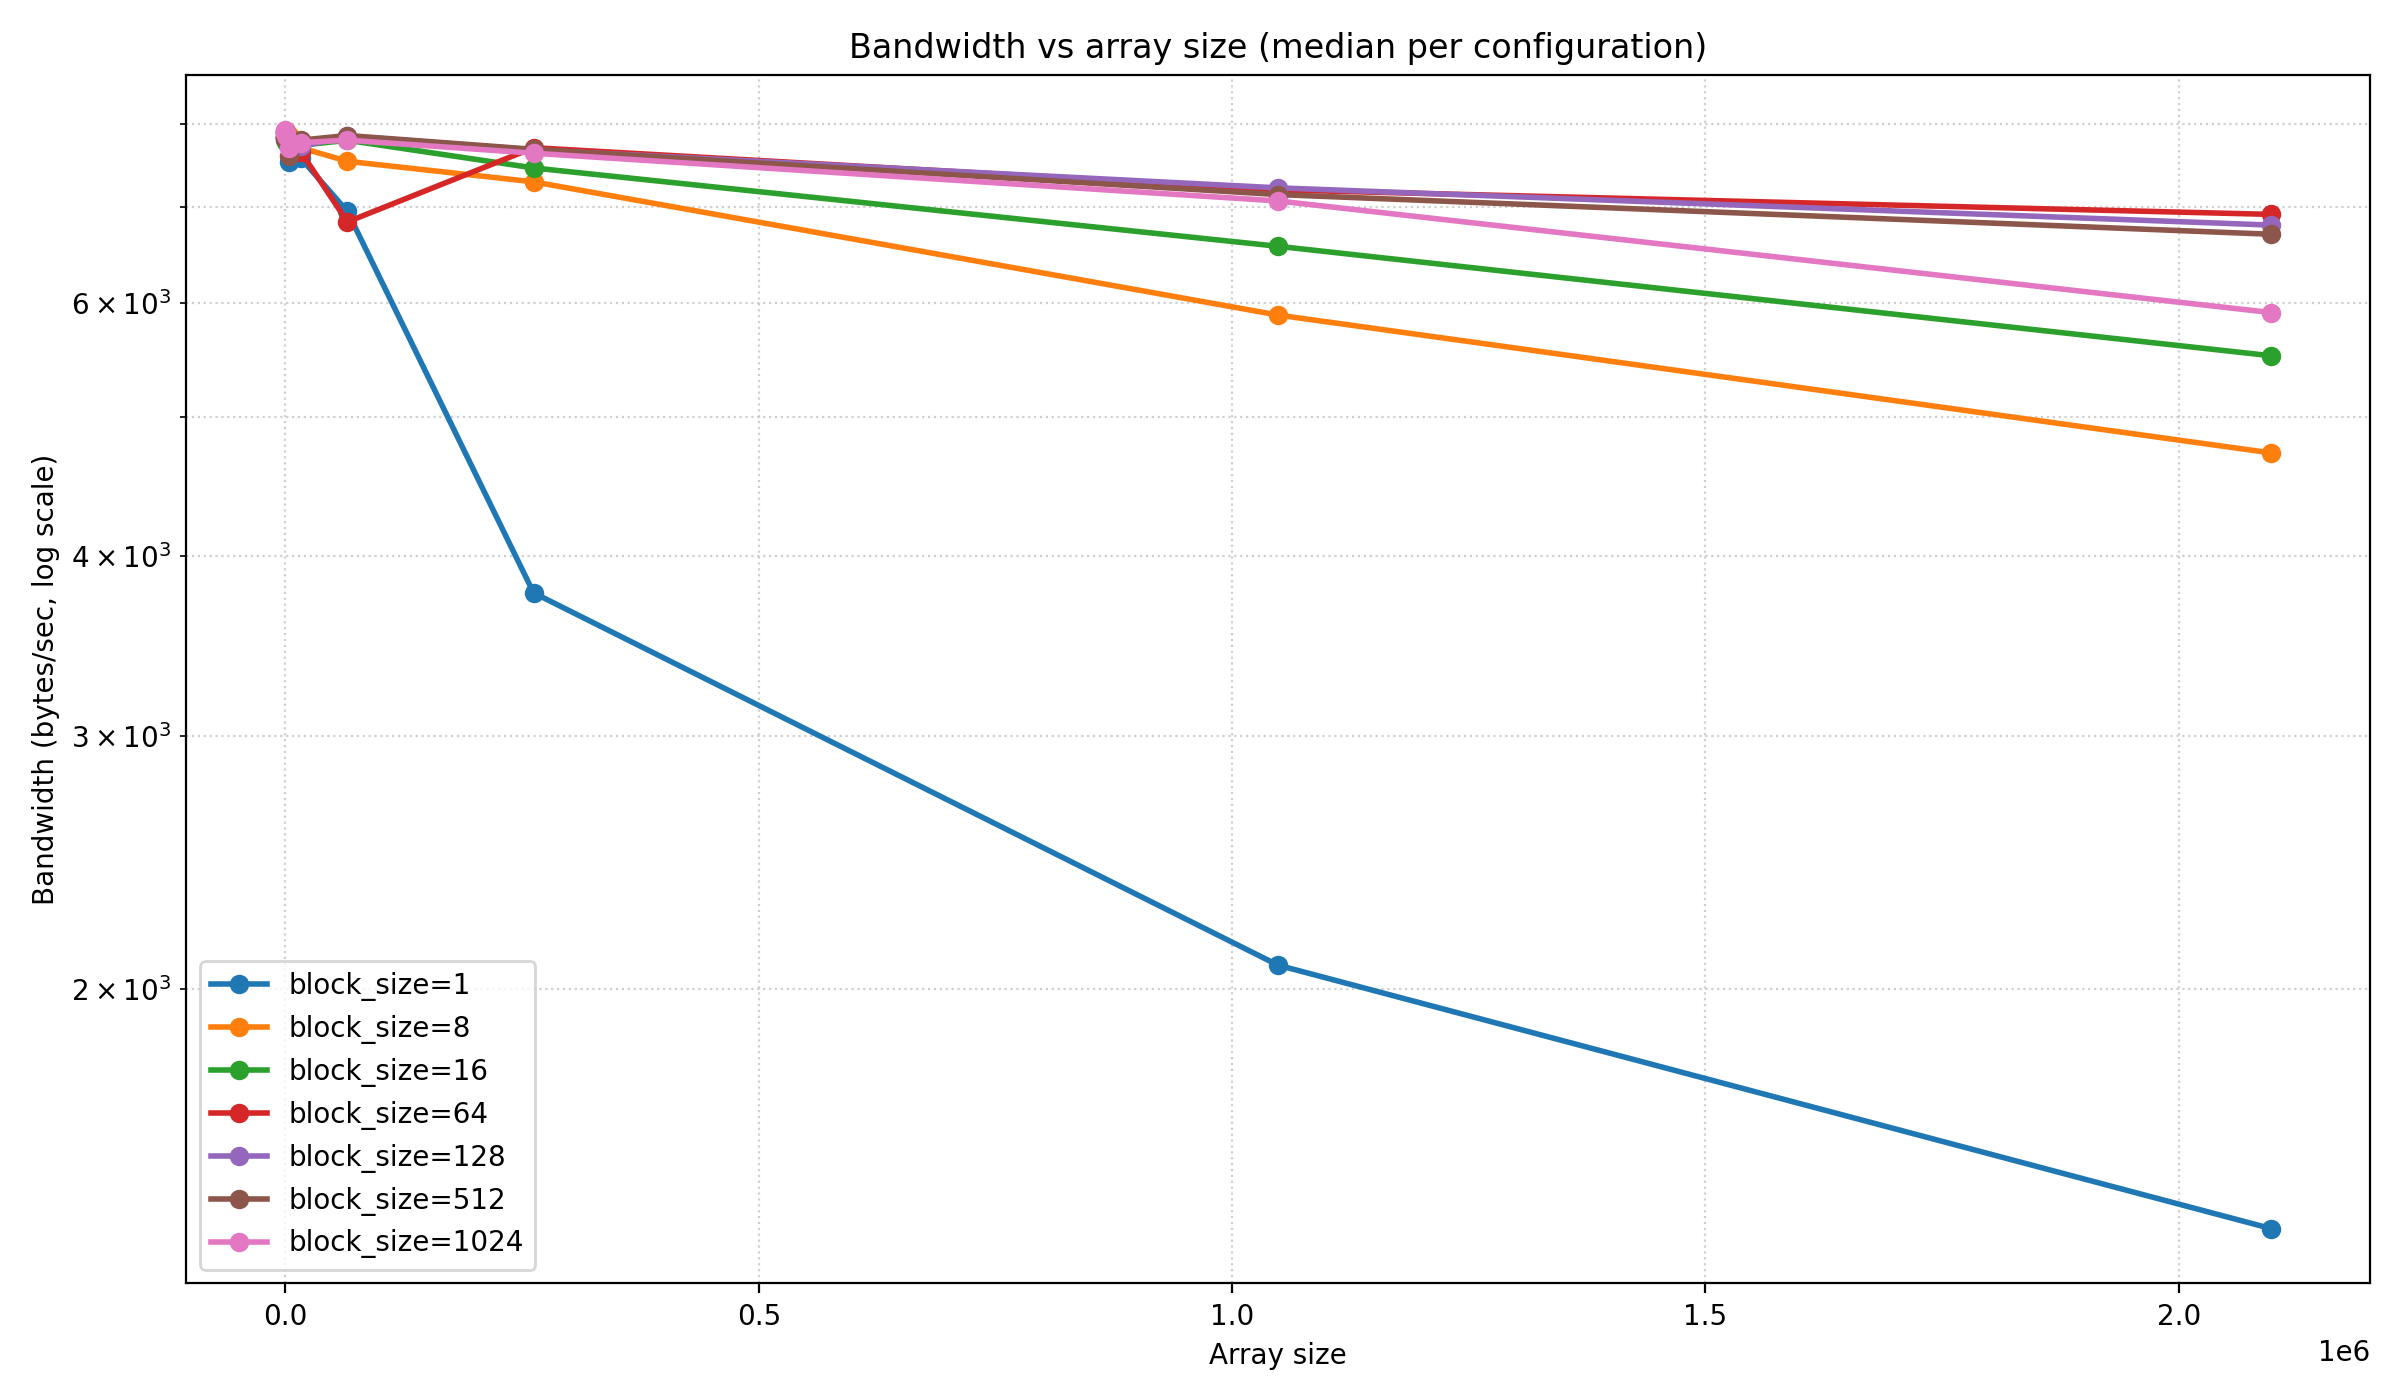
\includegraphics[width=1.0\textwidth]{../noah/plots/6_3/bandwidth_vs_array_size.png}
    \caption{CPU: Bandwith vs. size of data}
    \label{fig:3}
\end{figure}
\ref{fig:3} shows the bandwith of the kernel of the naive GPU implementation. Measurements are a done using a median value, since outliers where observed.\\
For smaller block sizes, perfomance drops significantly for larger matrices, since the CUDA cores are underutilized. For the largest blocksize of 1024, performance is slightly worse than for the 64-512 block sizes, which might be due to a reduced flexibility of scheduling warps and the necessity to synchronize the threads within a block.